The objective of this thesis is to investigate, how different energy storage models can be integrated into a microgrid co-simulation, which can simulate the energy system infrastructure of a data center. These models can range from simple, lossless batteries with the sole purpose of transferring usable energy over the duration of a simulation, to complex models of entire battery packs that take the internal physical processes of batteries as well as the energy losses of the battery packs circuit into account.

In addition to that, this work also proposes, how the important task of energy management in a microgrid environment can be simulated. This energy management can, for instance, include the charging and discharging of the microgrid's energy storage, the exchange of energy with the public utility grid, but also curtailment if there happens to be unusable excess energy.

The aim is to achieve this by extending the already existing co-simulation infrastructure of the Vessim framework \cite{vessim}, which has already been described in section \ref{vessim_infrastructure}, and add more context to specific parts of the design. Thereby, mainly the storage simulation unit is refined and explained in detail so that the described objectives can be met, and the infrastructure can be used as a co-simulation testbed for data centers. 

This chapter starts by outlining the used interface for the microgrid's energy storage in section \ref{energy_storage_interface}, which will be used to model battery packs at multiple levels of complexity. In section \ref{energy_management_policies}, it is discussed, how policies are defined, which are used to balance the energy within the microgrid at every time-step, and thus performing the necessary energy management. Finally, section \ref{extended_co-simulation_infrastructure} describes, how these components are integrated into the Vessim infrastructure, and how the energy and battery management can be tweaked during the simulation runtime.

\section{Energy Storage Interface}
\label{energy_storage_interface}
One of the main goals of this work is to describe a common interface for energy storage models to be used inside a microgrid co-simulation. This interface should be adaptable enough so that the complexity range of these models is not too limited, but has to be simple enough to allow a clear co-simulation infrastructure that still separates power consumption and power generation from the process of storing energy.

Similarly to what is described by Kazhamiaka et al. \cite{kazhamiaka2018pimodel} in their paper discussing the PI-model (see section \ref{c_l_c_model}), the input to the model is desired to be power instead of current. The reason for that is the underlying Vessim infrastructure \cite{vessim}, which conducts a power-flow analysis of the power network, as described in section \ref{vessim_infrastructure}, which would have to be transformed to obtain a charging or discharging current. Additionally, the management system should also be modeled as part of the energy storage system because the simulated battery should not be used in ways that would be prevented by a BMS (see section \ref{battery_management_systems}) like over- or undercharging.

In the proposed design, the \textit{Storage} provides the abstract interface for the management of an energy storage system, which allows for charging and discharging operations, and contains the monitoring and control functionality of a BMS. The primary function of the interface is to handle the energy flow into and from the battery, which is facilitated through an update method, receiving the power to be (dis-)charged $p_s$ as well as the (dis-)charging duration $d_s$. The \textit{Storage} adjusts its internal state based on these parameters, whereas the included BMS watches that the defined limits of the battery are respected. In the end, the function returns the total amount of energy $e_s$ that has been stored or discharged during this timeframe. For instance, if the battery was requested to charge at $p_s = 20W$ for $d = 10s$, but the BMS limits the charging to $15W$, the return value would be $e_s = 15W \cdot 10s = 150Ws$.

To allow for monitoring of the battery's internal state, a \textit{Storage} should also implement additional functionality. Discuss SoC and battery state.

\section{Energy Management Policies}
\label{energy_management_policies}
In the context of microgrid co-simulation, energy management is a critical part, as it has to be defined, how the microgrid responds to specific power deltas, which refer to the variations in power supply and demand. For this purpose, the approach allows for a user-defined \textit{MicrogridPolicy}, which provides a structured way to deal with these power fluctuations, whereas the management includes interactions with the public grid and present energy storage systems as well as curtailment.

The policy lets users define custom rules and strategies that balance the power delta of the microgrid's generators and consumers at every time-step. In case of excess power during the time-step, energy has to be stored, fed back to the utility grid, or curtailed, while a lack of power has to be leveled using either grid energy or the energy received by discharging the energy storage. These rules are applied at every time-step based on the current power delta and the duration that the delta is valid for.

When the \textit{MicrogridPolicy} is applied, it receives the current power delta $\Delta p$ (see section \ref{vessim_infrastructure}) and the time $d$ that passed since the last time-step. With the defined rules, the policy then decides, what portion of the power delta is to be balanced by charging or discharging the \textit{Storage} that the policy can access. It then instructs the \textit{Storage} to (dis-)charge with that power $p_s$ for a specified time $d_s$ that should be less or equal to $d$.

As discussed in section \ref{energy_storage_interface}, the \textit{Storage} returns the actual energy $e_s$ that could be charged or discharged given these inputs when it is updated. The policy finally uses that to compute the amount of energy $e$ that the microgrid has to draw or that the microgrid can feed into the public utility grid during the last time-step. The mentioned interactions between the \textit{MicrogridPolicy} and the \textit{Storage} is also depicted in figure \ref{fig:microgrid_policy}. In the most basic case, where no energy is curtailed, and the microgrid can exchange energy with the public grid at all times, the grid energy can be computed using the formula $e = \Delta p \cdot d - e_s$, where $\Delta p \cdot d$ marks the total energy surplus or deficit of the microgrid since the last time-step.

\begin{figure}[t]
    \centering
    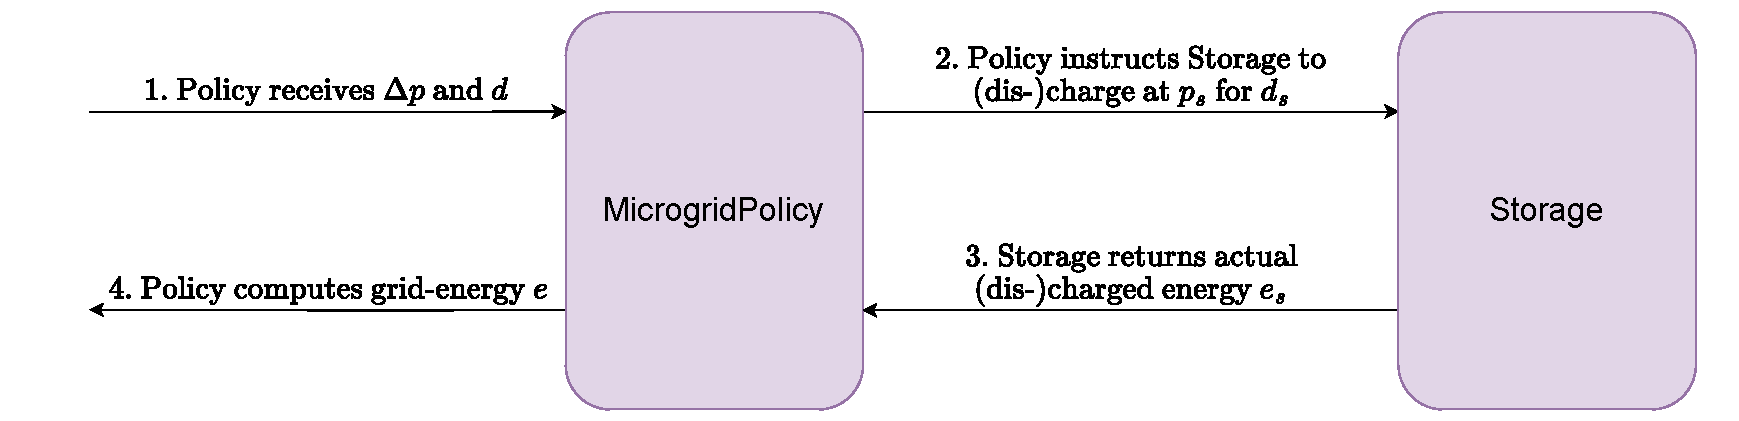
\includegraphics[width=\linewidth]{thesis/Images/Microgrid_Policy.pdf}
    \caption{Interaction between the \textit{MicrogridPolicy} and the \textit{Storage} during a simulation time-step.}
    \label{fig:microgrid_policy}
\end{figure}

\section{Extended Co-Simulation Infrastructure}
\label{extended_co-simulation_infrastructure}
\begin{figure}[t]
    \centering
    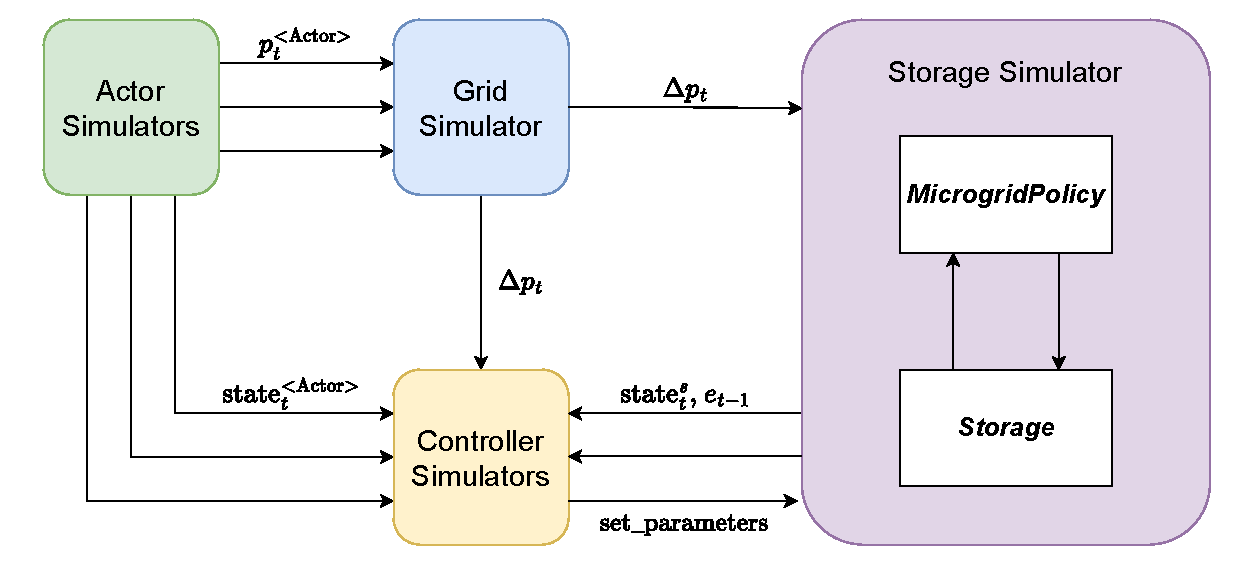
\includegraphics[width=\linewidth]{thesis/Images/Co_Simulation_Infrastructure.pdf}
    \caption{Refined Co-Simulation structure with the proposed energy storage interface.}
    \label{fig:co_simulation_infrastructure}
\end{figure}